% 我们为验证算法有效性做的实验

% 介绍dataset
% Dataset的生成方式
\begin{frame}{Experiment: Dataset Preparation}
    \begin{block}{Dataset}
    \begin{enumerate}
        \item Yelp Dataset: real world dataset
        \begin{enumerate}
        \item Phoenix
        \item Toronto
        \end{enumerate}
        
        \item Synthetic dataset, generated by different param-settings
        \begin{enumerate}
        \item Dataset 1 : Slack capacity constraints 
        \item Dataset 2 : balanced capacity constraints
        \item Dataset 3 : prominent capacity conflicts 
        \item Dataset 4 : serious capacity conflicts
        \end{enumerate}
        
    \end{enumerate}
    \end{block}
    \begin{block}{Evaluation Metric}

         \begin{enumerate}
        \item Total quality of recommendations of each user
        \item Variance among Top-N Fairness of all users
        \end{enumerate}

    
        \end{block}
    
\end{frame}





% 介绍使用到对比的另两种方法
\begin{frame}{Experiment: Constrast Algorithms}
    We compare our algorithm against the following two baseline methods
    
    \begin{block}{Preempt Strategy}
A kind of first-come first-served (FCFS) process scheduling algorithm which doesn’t take fairness into consideration
    
        \end{block}
        \begin{block}{Random Strategy}
Assign Services to users randomly, which can also assure Top-N Fairness in the long run.
        \end{block}
    
\end{frame}




% 分别介绍真实数据集和人工数据集的实验情况,插入图表
\begin{frame}{Experiment on Yelp Dataset}


\begin{figure}[htbp]
\centering
\subfigure{
\begin{minipage}[t]{0.36\linewidth}
\centering
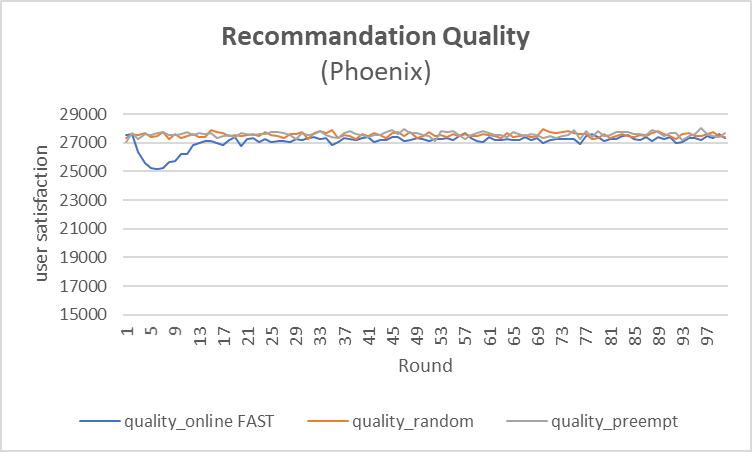
\includegraphics[width=1.6in]{img/2_q_p.png}
\end{minipage}%
}%
\subfigure{
\begin{minipage}[t]{0.36\linewidth}
\centering
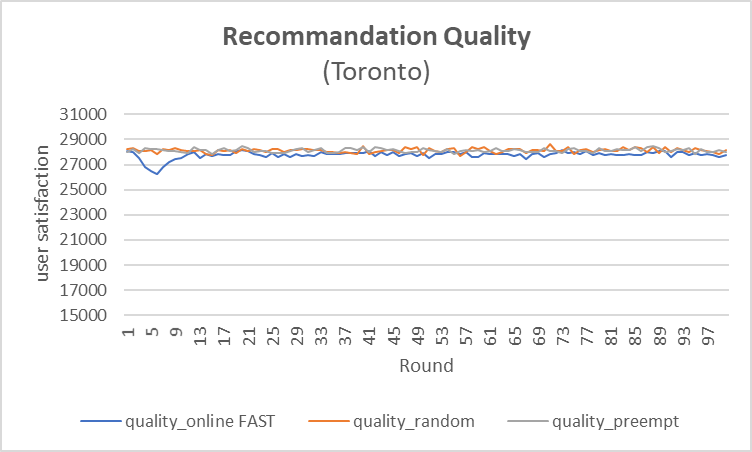
\includegraphics[width=1.6in]{img/2_q_t.png}
\end{minipage}%
}%
\caption{Online FAST keeps Recommendation Quality at a high level}
\end{figure}

\begin{figure}
\subfigure{
\begin{minipage}[t]{0.36\linewidth}
\centering
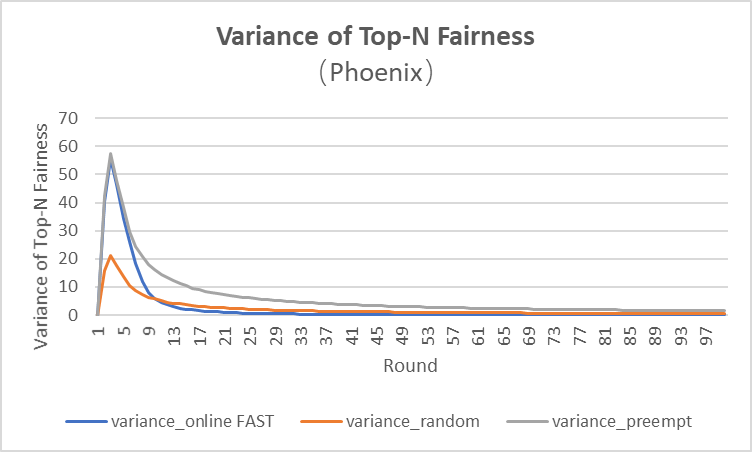
\includegraphics[width=1.6in]{img/2_v_p.png}
\end{minipage}
}%
\subfigure{
\begin{minipage}[t]{0.36\linewidth}
\centering
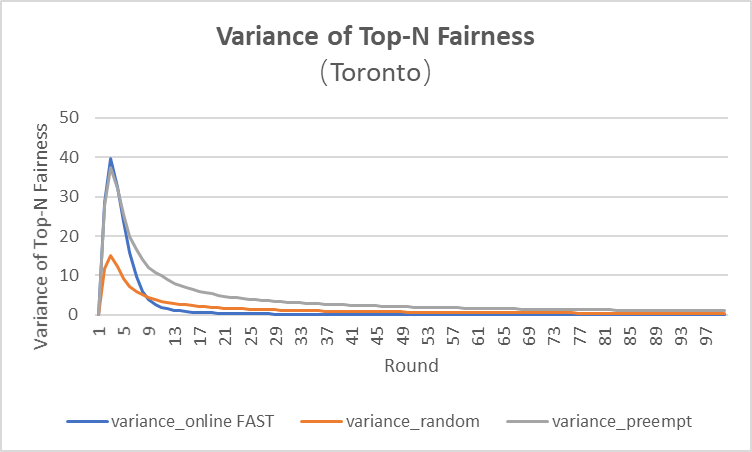
\includegraphics[width=1.6in]{img/2_v_t.png}
\end{minipage}
}%
\centering
\caption{Online FAST shows better convergence property (Arrival Probability = 0.8, N = 5)}
\end{figure}
\end{frame}


\begin{frame}{Experiment on Synthetic Dataset }

\begin{figure}[htbp]
\centering
\subfigure[Dataset 1]{
\begin{minipage}[t]{0.36\linewidth}
\centering
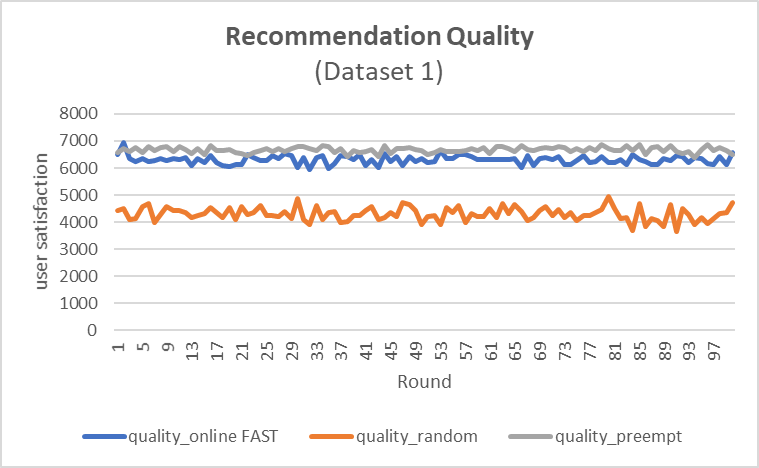
\includegraphics[width=1.6in]{img/1_q_1.png}
\end{minipage}%
}%
\subfigure[Dataset 2]{
\begin{minipage}[t]{0.36\linewidth}
\centering
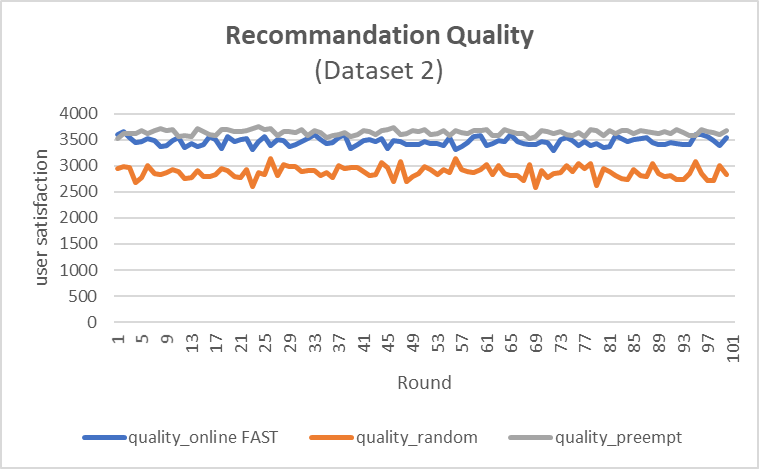
\includegraphics[width=1.6in]{img/1_q_2.png}
\end{minipage}%
}%

\subfigure[ Dataset 3]{
\begin{minipage}[t]{0.36\linewidth}
\centering
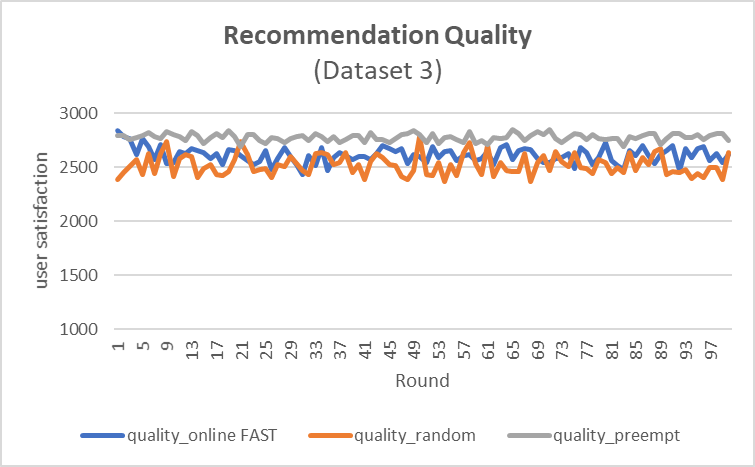
\includegraphics[width=1.6in]{img/1_q_3.png}
\end{minipage}
}%
\subfigure[Dataset 4]{
\begin{minipage}[t]{0.36\linewidth}
\centering
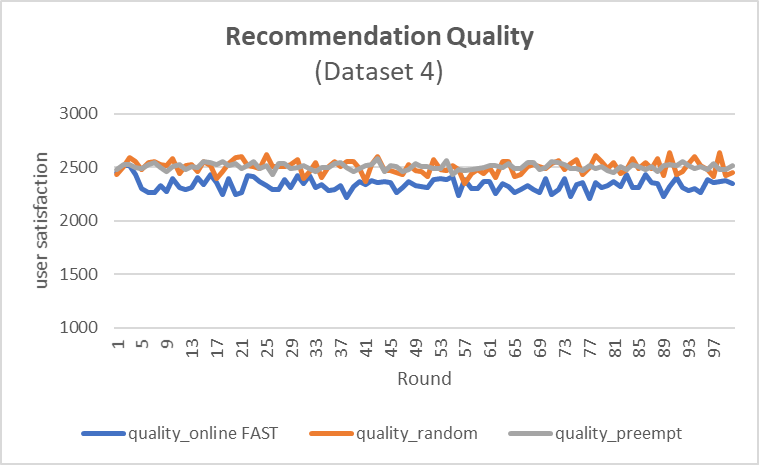
\includegraphics[width=1.6in]{img/1_q_4.png}
\end{minipage}
}%
\centering
\caption{Recommendation Quality of Online-FAST is steady under different levels of capacity constraints\ (Arrival Probability = 0.6, N = 5)}
% \label{fig:RQ}
\end{figure}
\end{frame}


\begin{frame}{Experiment on Synthetic Dataset}

\begin{figure}[htbp]
\centering
\subfigure[Dataset 1]{
\begin{minipage}[t]{0.36\linewidth}
\centering
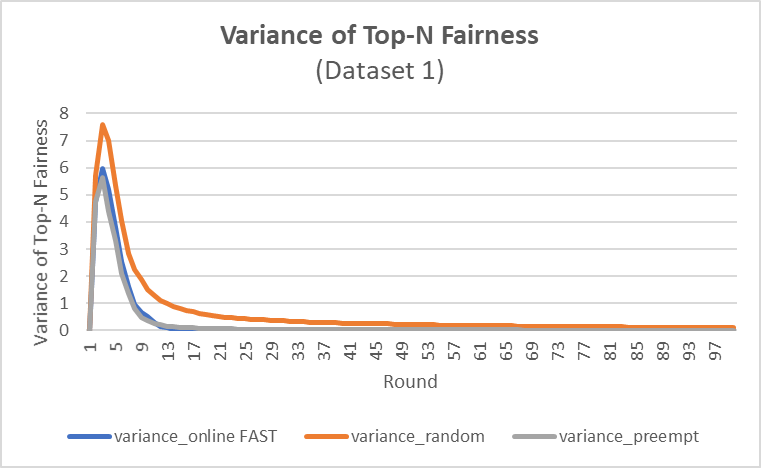
\includegraphics[width=1.6in]{img/1_v_1.png}
\end{minipage}%
}%
\subfigure[Dataset 2]{
\begin{minipage}[t]{0.36\linewidth}
\centering
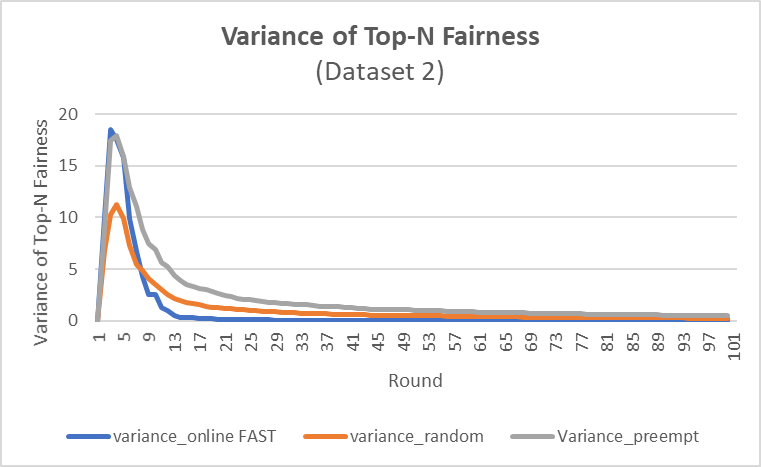
\includegraphics[width=1.6in]{img/1_v_2.png}
\end{minipage}%
}%

\subfigure[ Dataset 3]{
\begin{minipage}[t]{0.36\linewidth}
\centering
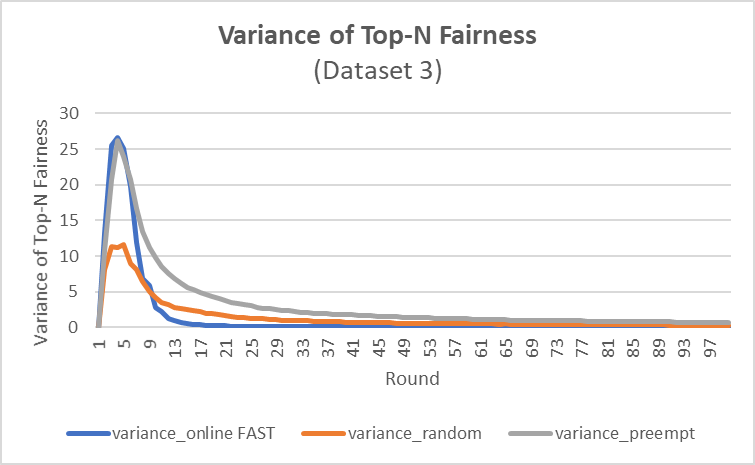
\includegraphics[width=1.6in]{img/1_v_3.png}
\end{minipage}
}%
\subfigure[Dataset 4]{
\begin{minipage}[t]{0.36\linewidth}
\centering
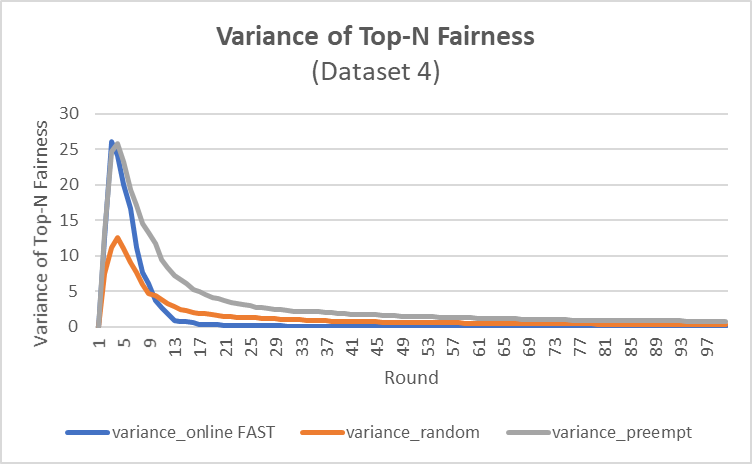
\includegraphics[width=1.6in]{img/1_v_4.png}
\end{minipage}
}%
\centering
\caption{Variance of Top-N Fairness can converge under different levels of capacity constraints (Arrival Probability = 0.6, N = 5)}
\end{figure}
\end{frame}


\begin{frame}{Experiment on Synthetic Dataset}

\begin{figure}[htbp]
\centering
\subfigure[P=0.5]{
\begin{minipage}[t]{0.36\linewidth}
\centering
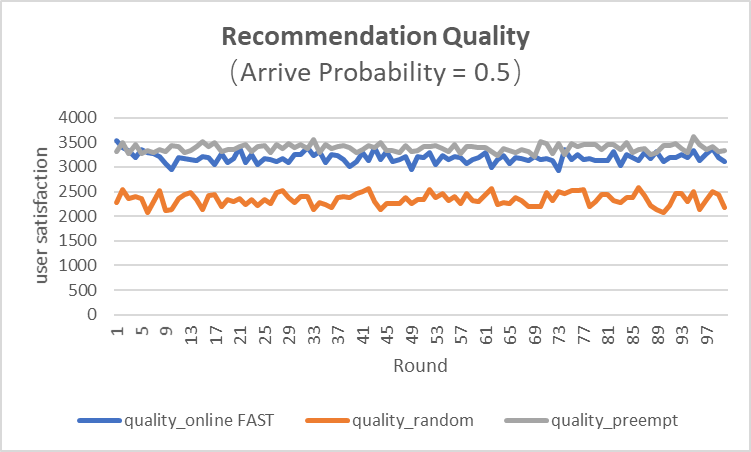
\includegraphics[width=1.6in]{img/3_q_0.5.png}
\end{minipage}%
}%
\subfigure[P=0.6]{
\begin{minipage}[t]{0.36\linewidth}
\centering
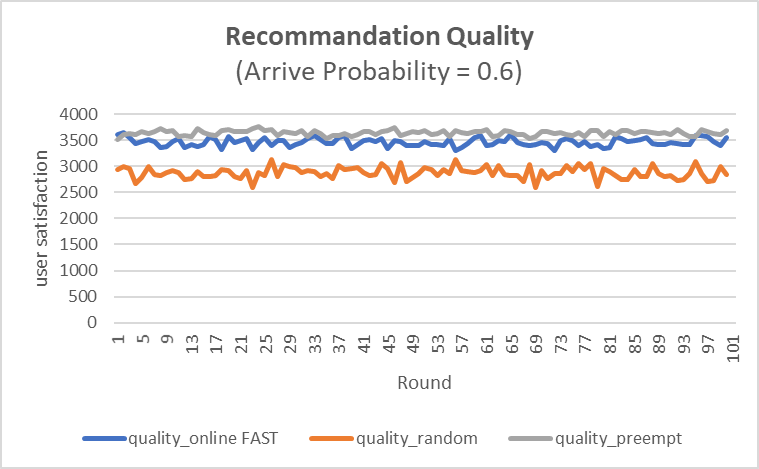
\includegraphics[width=1.6in]{img/3_q_0.6.png}
\end{minipage}%
}%

\subfigure[P=0.7]{
\begin{minipage}[t]{0.36\linewidth}
\centering
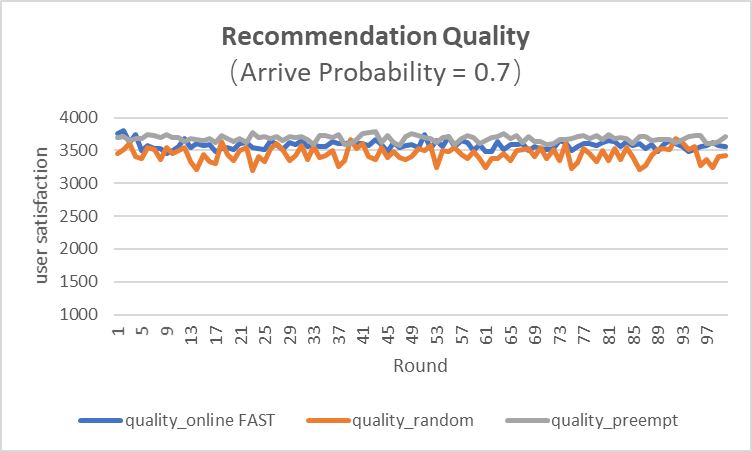
\includegraphics[width=1.6in]{img/3_q_0.7.png}
\end{minipage}
}%
\subfigure[P=0.8]{
\begin{minipage}[t]{0.36\linewidth}
\centering
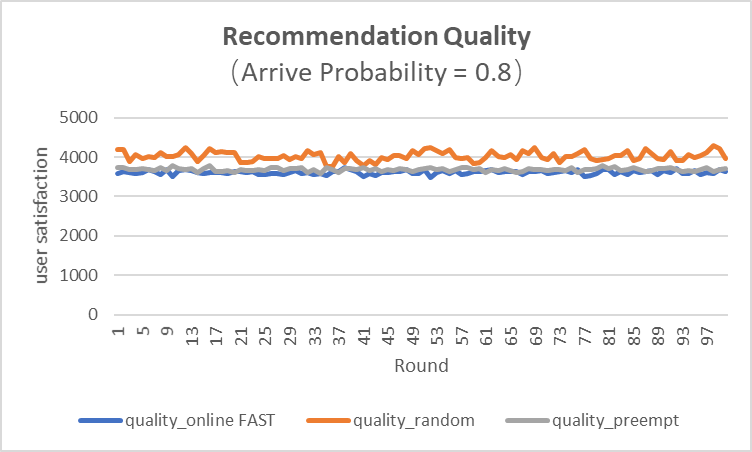
\includegraphics[width=1.6in]{img/3_q_0.8.png}
\end{minipage}
}%
\centering
\caption{Recommendation Quality is steady under different arriving probability  (on Balanced Capacity Constraints Dataset, N = 5)}
\end{figure}
\end{frame}





